\clearpage
\VerdierPhysicalPageAnchor{0141}%
\begingroup
\small
\setlength{\parskip}{0pt}%
\setlength{\emergencystretch}{1.5em}%
\setlength{\abovedisplayskip}{1pt plus 1pt minus 1pt}%
\setlength{\belowdisplayskip}{1pt plus 1pt minus 1pt}%

\VerdierSemanticAnchor{ch2-2-2-8-stepwise-conditions}
\noindent such that:

\VerdierSemanticAnchor{ch2-2-2-8-condition-1}
\par\noindent\makebox[1.8em][l]{1)}$us_1=tu_1''$ and $s_1\in S$.
This is done using SM2).

\VerdierSemanticAnchor{ch2-2-2-8-condition-2}
\par\noindent\makebox[1.8em][l]{2)}$mQ(s_1s_2)=Q(f')$, where
$f'\colon X_2''\longrightarrow X'$ is a morphism of $\mathcal D$,
$u_2''=u_1''s_2$, and $s_2\in S$. This is done using theorem (2.2.2).

\VerdierSemanticAnchor{ch2-2-2-8-condition-3}
\par\noindent\makebox[1.8em][l]{3)}$u'f's_3=gu_2''s_3$,
$u''=u_2''s_3$, and $s_3\in S$. Indeed, the diagram in $\mathcal D$:

\VerdierSemanticAnchor{ch2-2-2-8-source-square}
\begin{center}
  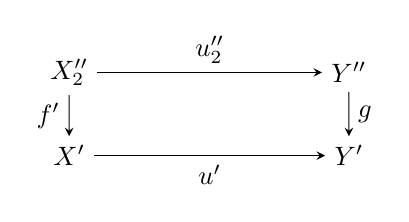
\begin{tikzpicture}[>=stealth,line width=.38pt,x=1.85cm,y=1.10cm,
    scale=.96,transform shape]
    \node (X2pp) at (0,1) {$X_2''$};
    \node (Ypp)  at (2,1) {$Y''$};
    \node (Xp)   at (0,0) {$X'$};
    \node (Yp)   at (2,0) {$Y'$};
    \draw[->] (X2pp) -- node[above] {$u_2''$} (Ypp);
    \draw[->] (X2pp) -- node[left] {$f'$} (Xp);
    \draw[->] (Ypp)  -- node[right] {$g$} (Yp);
    \draw[->] (Xp)   -- node[below] {$u'$} (Yp);
  \end{tikzpicture}
\end{center}

\VerdierSemanticAnchor{ch2-2-2-8-localized-commutativity}
\noindent is not necessarily commutative. But the diagram in
$\mathcal D(S^{-1})$ obtained by applying the functor $Q$ to the preceding
diagram is commutative. We therefore have
$Q(u'f')=Q(gu_2'')\colon Q(X_2'')\longrightarrow Q(Y')$.

\VerdierSemanticAnchor{ch2-2-2-8-s3-refinement}
It follows, by the definition of the morphisms of $\mathcal D(S^{-1})$,
that there exists a morphism
$s_3\in S\colon X''\longrightarrow X_2''$ such that
$u'f's_3=gu_2''s_3$.

\VerdierSemanticAnchor{ch2-2-2-8-proof-complete}
To complete the proof of the lemma, it suffices to set
$f=f's_3$, $s=s_1s_2s_3$.

\VerdierSemanticAnchor{ch2-2-2-9}
\smallskip
\noindent\textbf{2.2.9. Completion of the proof of theorem 2.2.6.}
\VerdierSemanticAnchor{ch2-2-2-9-triv-reduction}%
It remains to prove that the set $T$ has property TRIV. We now know that
this set has properties TRI, TRII, and TRIII. We may therefore use the
results of 1.2 (1.2.14). In particular, it follows from (1.2.4) that all
triangles in $T$ containing a given morphism are isomorphic. Thus, by
reductions analogous to those used in the proof of proposition (1.3.2),
the proof of property TRIV may be reduced to diagrams in
$\mathcal D(S^{-1})$ that are images under $Q$ of analogous diagrams in
$\mathcal D$.

\VerdierSemanticAnchor{ch2-2-2-9-reader-details}
The verification is then easy. We leave the details to the reader.

\VerdierSemanticAnchor{ch2-2-2-10}
\smallskip
\noindent\textbf{2.2.10.}\quad
Let $\mathcal D$ be a triangulated category,
$\mathcal B\subseteq\mathcal D$ a full triangulated subcategory, and
$S(\mathcal B)$ the multiplicative system associated with $\mathcal B$
(2.1.15).

\VerdierSemanticAnchor{ch2-2-2-10-quotient-category}
We denote by $\mathcal D/\mathcal B$ the category
$\mathcal D(S(\mathcal B)^{-1})$. The category $\mathcal D/\mathcal B$
is called the \emph{quotient category of $\mathcal D$ by $\mathcal B$}.

\VerdierSemanticAnchor{ch2-2-2-10-quotient-functor}
The canonical functor
$Q\colon\mathcal D\longrightarrow\mathcal D/\mathcal B$ is called the
\emph{quotient functor}. Let
$F\colon\mathcal D\longrightarrow\mathcal D'$ be an exact
(resp. cohomological) functor into a triangulated (resp. abelian) category.

\VerdierSemanticAnchor{ch2-2-2-10-kernel}
We denote by $\operatorname{Ker}(F)$, and call the \emph{kernel of $F$},
the strictly full saturated triangulated subcategory defined by the
objects carried by $F$ to zero objects (resp. whose translates are all
carried by $F$ to zero objects) ((2.1.16) and (2.1.17)).

\VerdierSemanticAnchor{ch2-2-2-10-p142-boundary}
\endgroup

